%!TEX TS-program = xelatex
\documentclass{mycv}

%%%%% LANGUAGE AND FONTS 
\usepackage{xltxtra,xgreek,fontspec} 			 
\setmainfont{Times New Roman}            % main font
%\setmonofont{Courier New}		 % for commands
\usepackage[greek]{datetime2} 		 % show greek date correctly using \today command
\renewcommand{\today}{\ifcase\month\or%
	Ιανουάριος\or Φεβρουάριος\or Μάρτιος\or% 
	Απρίλιος\or Μάιος\or Ιούνιος\or Ιούλιος%
	\or Αύγουστος\or Σεπτέμβριος\or% 
	Οκτώβριος\or Νοέμβριος\or% 
	Δεκέμβριος\fi\ \number \year}			 % nominative instead of genitive 

\hypersetup{%
  pdftitle={Χρήστος Δαλαμάγκας - Βιογραφικό},
  pdfauthor={Χρήστος Δαλαμάγκας},
  pdfsubject={Βιογραφικό},
  pdfkeywords={Χρήστος Δαλαμάγκας, Christos Dalamagkas}
}

\begin{document}
	\thispagestyle{plain}
	\begin{minipage}{.7\textwidth}
		\begin{flushleft}
			\name{Χρήστος Δαλαμάγκας}{Βοηθος Ερευνας}{Μηχανικος Δικτυων (CCNA)}
			\contact{(+30) 698 316 0295}{cdalamagkas@gmail.com}{chris.dal}{https://christos.pw}{linkedin.com/in/cdalamagkas}{cdalamagkas}
			\centering
			{\bf Ημερομηνία Γέννησης}: 3 Νοεμβρίου 1994
		\end{flushleft}
	\end{minipage}
	\begin{minipage}{.3\textwidth}
		\begin{flushright}
			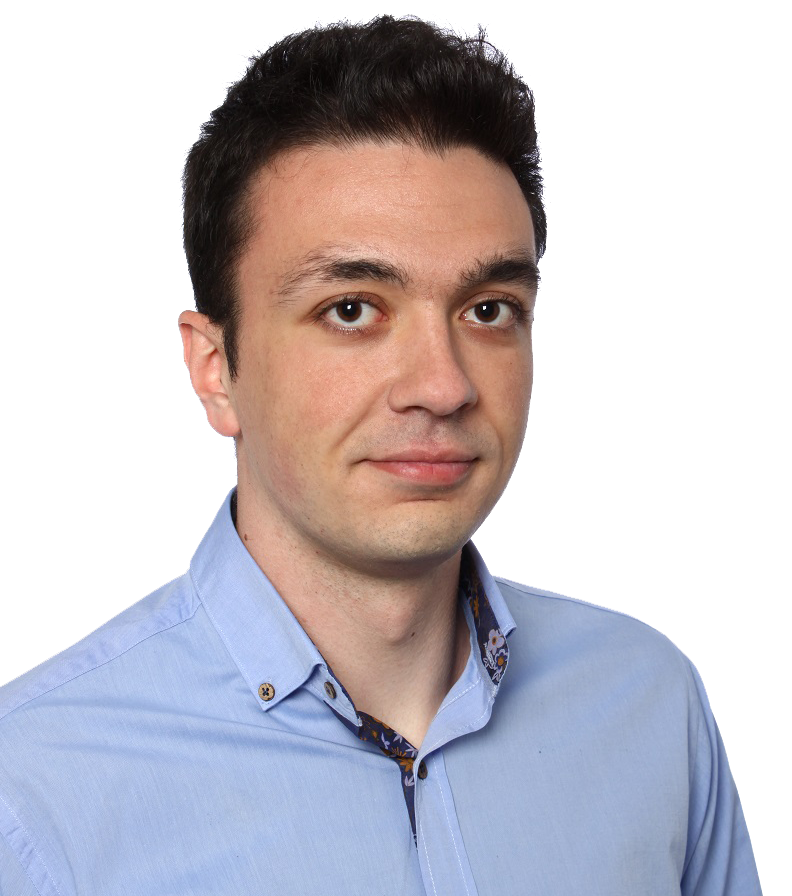
\includegraphics[scale=0.2]{assets/photo.jpg}
		\end{flushright}
	\end{minipage}
	%
	%\vspace*{-0.5cm}
	%
	\section{Εκπαιδευση}
	
	\begin{EntryDatedLogo}{Πανεπιστήμιο Δυτικής Μακεδονίας}{http://ece.uowm.gr}{2012 -- 2017}{Διπλωμα (Πενταετους φοιτησης), Πρ. Τμημα Μηχανικων Πληροφορικης και Τηλεπικοινωνιων}{-1.25cm}{uowm}{0.6}
		\begin{Itemize}
			%\item Recognized as integrated master degree (level 7 of EFQ) under government gazette 3987/14-9-2018
			%\item Thesis title: "\textit{Design of Market Mechanism for Dynamic Bandwidth Allocation on XG-PON}".
			\item Θεωρία παιγνίων στα δίκτυα XG-PON: \url{https://christos.pw/thesis}.
			\item Βαθμός αποφοίτησης: 8.2/10.
		\end{Itemize}
	\end{EntryDatedLogo}
	
	\section{Επαγγελματικη εμπειρια}
	\begin{EntryDatedLogo}{Δημόσια Επιχείρηση Ηλεκτρισμού}{https://www.dei.gr/en}{Μάϊ. 2018 - Τώρα}{Βοηθος Ερευνας}{-1.25cm}{dei}{0.6}
	\begin{Itemize}
		\item Ερευνητής σε προγράμματα Ορίζοντα 2020 (SPEAR, SDN-microSENSE).
		\item Έξυπνα δίκτυα ηλεκτρικής ενέργειας, βιομηχανικά δίκτυα και κυβερνοασφάλεια.
	\end{Itemize}
	\end{EntryDatedLogo}

	\vspace*{0.5cm}

	\begin{EntryDatedLogo}{Ελεύθερος Επαγγελματίας - Μηχανικός ICT}{https://christos.pw}{Jun. 2018 - Τώρα}{Μηχανικος L1}{-1cm}{engineer}{0.6}
		\begin{Itemize}
			\item Εργολήπτης μηχανικός δικτύων με πιστοποίηση CCNA.
			\item Μηχανικός πεδίου συνεργαζόμενος με εταιρίες IT (NSC Global)
		\end{Itemize}
	\end{EntryDatedLogo}

	\vspace*{0.5cm}	

	\begin{EntryDatedLogo}{Πανεπιστήμιο Δυτικής Μακεδονίας}{https://ece.uowm.gr}{Μάρ. 2017 - Τώρα}{Βοηθος ερευνας}{-1cm}{uowm}{0.6}
		\begin{Itemize}
			\item Βοηθός εργαστηρίου στα Δίκτυα Υπολογιστών, Κυβερνοασφάλεια και προσομοίωση.
			\item Έρευνα για προετοιμασία ερευνητικών προτάσεων και εκτέλεσης ευρωπαϊκών προγραμμάτων Ορίζοντα 2020.
			\item Προγραμματιστής (Εφαρμογές ιστού και SDN).
		\end{Itemize}
	\end{EntryDatedLogo}
	
	\vspace*{0.5cm}
	
	\begin{EntryDatedLogo}{ΙΙΕΚ ΑΛΦΑ}{https://iekalfa.gr}{Οκτ. 2018 - Ιουν. 2019}{Δασκαλος}{-1cm}{alfa}{0.6}
		\begin{Itemize}
			\item Δίκτυα υπολογιστών και τηλεπικοινωνίες.
			\item Λειτουργικά Συστήματα και Αντικειμενοστραφής Προγραμματισμός (C++).
		\end{Itemize}
	\end{EntryDatedLogo}

	\vspace*{0.5cm}
		
	\begin{EntryDatedLogo}{Πανεπιστήμιο του Brighton}{https://www.brighton.ac.uk}{Ιουλ. - Σεπτ. 2017}{Βοηθος Ερευνας}{-0.45cm}{brighton}{0.6}
	\end{EntryDatedLogo}

	\vspace*{0.75cm}	

	\begin{EntryDatedLogo}{IntelliSolutions S.A}{http://intelli-corp.com}{Ιούλ. - Αυγ. 2016}{Μηχανικος Δικτυων και Συστηματων (Ασκουμενος)}{-0.4cm}{intelli}{0.75}
	\end{EntryDatedLogo}
	\newpage
	
	\section{Επαγγελματικες Πιστοποιησεις}
	\begin{EntryDatedLogo}{Cisco Certified Network Associate (CCNA)}{https://www.cisco.com/}{\scshape{Ιουλ. 2019}}{Σε ισχυ}{-0.75cm}{cisco}{0.6}
	\end{EntryDatedLogo}
	\vspace{0.25cm}
	
	\section{Δεξιοτητες}
	\begin{tabular}{m{4.5cm} m{13cm}}\renewcommand{\arraystretch}{2}
		\textbf{Τηλεπικοινωνίες}   		& ITU-T PONs, Traffic Engineering, Simulation (OmNET++). \\
		\textbf{Δικτύωση}   			& Ύλη του CCNA, Open vSwitch, RouterOS, ArubaOS, OpenFlow, προγραμματισμός SDN.\\
		\textbf{Ασφάλεια}				& TLS, PKI, OpenVPN, pfSense, ACLs και Firewall. \\
		\textbf{Διαχείριση Συστημάτων}	& Unix, LEMP stack, Windows Server, Active Directory. \\
		\textbf{Εικονικοποίηση}			& Xen (XCP-ng), ESXi, Proxmox VE, VMware/VirtualBox, Docker.\\ 
		\textbf{Προγραμματισμός} 	    & Java, MATLAB, Python, C/C++, Προγραμματισμός Ιστού, Django. \\
		\textbf{Διάφορα}				& Troubleshooting, Project Management, Office Suite, MS Visio, \LaTeX. \\
		\textbf{Γλώσσες} 				& Greek (εγγενώς), English (C2), German (C1). 
	\end{tabular}

	\section{Εθελοντικες Δραστηριοτητες και Συνδρομες}
	\vspace*{0.125cm}	
	\begin{EntryDatedLogo}{Πανεπιστήμιο Δυτικής Μακεδονίας}{https://uowm.gr}{Μαρτ. 2016 - Τώρα}{Συντακτης εκπαιδευτικου υλικου}{-1.1cm}{uowm}{0.6}
		\begin{Itemize}
			\item Συγγραφή πρωτότυπου εκπαιδευτικού υλικού για το μάθημα «Σχεδίαση Δικτύων».
			\item Η ύλη περιλαμβάνει δρομολόγηση και μεταγωγή με συσκευές Cisco και Mikrotik.
		\end{Itemize}
	\end{EntryDatedLogo}
	
	\vspace*{0.5cm}
	
	\begin{EntryDatedLogo}{Ινστιτούτο Ηλεκτρολόγων και Ηλεκτρονικών Μηχανικών}{https://www.ieee.org/}{Σεπτ. 2013 -- Τώρα}{Μελος της κοινοτητας IEEE Communications}{-0.5cm}{ieee}{0.6}
	\end{EntryDatedLogo}
	
	\section{Δημοσιευσεις}
	\pubentry{1}{C. Dalamagkas, P. Sarigiannidis, S. Kapetanakis and I. Moscholios, "Dynamic scheduling in {TWDM}-{PONs} using game theory", \textit{Optical Switching and Networking}, Dec. 2017, DOI: \href{https://doi.org/10.1016/j.osn.2017.12.004}{\texttt{10.1016/j.osn.2017.12.004}}.}{2018}
	
	\pubentry{2}{C. Dalamagkas, P. Sarigiannidis, I. Moscholios, T. Lagkas and M.S. Obaidat, "PAS: A Fair Game-Driven DBA Scheme for XG-PON Systems", \textit{11th International Symposium on Communication Systems, Networks, and Digital Signal Processing}, Jul. 2018. DOI: 
	\href{https://doi.org/10.1109/CSNDSP.2018.8471787}{\texttt{10.1109/CSNDSP.2018.8471787}}}{2018}
	
	\pubentry{3}{C. Dalamagkas et al., “A Survey On Honeypots, Honeynets And Their Applications On Smart Grid,” in 2019 IEEE Conference on Network Softwarization (NetSoft), 2019. DOI: 
	\href{http://dx.doi.org/10.1109/NETSOFT.2019.8806693}{\texttt{10.1109/NETSOFT.2019.8806693}}}{2019}
	
	\pubentry{4}{P. Diamantoulakis, C. Dalamagkas, P. Radoglou-Grammatikis, P. Sarigiannidis, and G. Karagiannidis, “Game Theoretic Honeypot Deployment in Smart Grid,” Sensors, vol. 20, no. 15, p. 4199, Jul. 2020. DOI: \href{http://dx.doi.org/10.3390/s20154199}{\texttt{10.3390/s20154199}}}{2020}
	
	\vspace{-0.25cm}

\end{document}
